\chapter{Общее уравнение динамики в обобщенных координатах. Уравнения Лагранжа
2-го рода. Примеры применения уравнений Лагранжа в потенциальном поле сил.}

Рассмотрим систему из \( n \) материальных точек с идеальными связями. Для неё
справедливо общее уравнение динамики:
\[
    \sum\limits_{j=1}^n \underbrace{\delta A^e_j}_{
        \substack{\textbf{работа} \\ \textbf{силовых полей}}    
        }
    +
    \sum\limits_{j=1}^n\underbrace{ \delta A^\text{и}_j}_{
            \substack{\textbf{работа} \\ \textbf{силы инерции}}
            }   
    = 0,
\]
где 
\[
    \delta A^e_j = \vec{F}_{j} \cdot \delta \vec{r}_{j},\quad
    \delta A^\text{и}_n = \vec{\text{Ф}}_{j}\cdot\delta\vec{r}_{j},
\]
\( \vec{F}_{j} \) -- силовые поля, действующие на \( i \) материальную точку,
\( \vec{\text{Ф}}_{j} = - m_j \der{\vec{v}_{j}}{t} \) -- силы инерции.

Радиус-вектор \( j \) материальной точки в зависимости от обобщённых координат
\( (q_1, q_2, ... q_s) \) и времени:
\[
    \vec{r}_{j} = \vec{r}_{j}(q_1, q_2, ... q_s, t).
\]
Тогда
\[
    \delta  \vec{r}_{j} = \sum\limits_{i=1}^s\pder{\vec{r}_{j}}{q_i} \delta q_i.
\]

Кроме того, дифференцируя \( \vec{r}_{j} \) по \( t \), получим
\[
    \vec{v}_{j} = \der{\vec{r}_{j}}{t} = 
    \sum\limits_{i=1}^s \pder{\vec{r}_{j}}{q_i} \dot{q}_i +
    \pder{\vec{r}_{j}}{t},
\]
откуда учитывая, что \( \vec{r}_{j} \) не зависит от \( \dot{q}_i \),
получим первое тождество Лагранжа:
\[
    \pder{\vec{v}_{j}}{\dot{q}_i} =
    \pder{\vec{r}_{j}}{q_i}.
\]

Дифференцируя \( \pder{\vec{r}_{j}}{q_i} \) по времени
\[
    \der{}{t}\left(\pder{\vec{r}_{j}}{q_i}\right) =
    \sum\limits_{k=1}^s
    \ppder{\vec{r}_{j}}{q_i \partial q_k} \dot{q}_k +
    \ppder{\vec{r}_{j}}{q_i \partial t}
\]
и сравнивая с выражением
\[
    \pder{\vec{v}_{j}}{q_i} =
    \sum\limits_{k=1}^s
    \ppder{\vec{r}_{j}}{q_i \partial q_k} \dot{q}_k +
    \ppder{\vec{r}_{j}}{q_i \partial t},
\]
получим второе тождество Лагранжа:
\[
    \der{}{t}\left(\pder{\vec{r}_{j}}{q_i}\right) =
    \pder{\vec{v}_{j}}{q_i}.
\]
    
Далее   
\begin{gather*}
    \sum\limits_{j=1}^n \delta A^e_j =
    \sum\limits_{j=1}^n \vec{F}_{j} \cdot \delta \vec{r}_{j} =
    \sum\limits_{j=1}^n \vec{F}_{j} \cdot
    \sum\limits_{i=1}^s\pder{\vec{r}_{j}}{q_i} \delta q_i =
    \sum\limits_{j=1}^n \sum\limits_{i=1}^s 
    \left(\vec{F}_{j} \cdot \pder{\vec{r}_{j}}{q_i}
    \right)
    \delta q_i = \\ =
    \sum\limits_{i=1}^s  
    \left(
    \sum\limits_{j=1}^n 
    \vec{F}_{j} \cdot \pder{\vec{r}_{j}}{q_i}
    \right)
    \delta q_i.
\end{gather*}
Но по определению
\( \sum\limits_{j=1}^n \vec{F}_{j}\cdot\pder{\vec{r}_{j}}{q_i} = Q_i \)~--
обобщённые силы.
\[
    \sum\limits_{j=1}^n \delta A^e_j = \sum\limits_{i=1}^s  Q_i\delta q_i, 
\]
\begin{gather*}
    \sum\limits_{j=1}^n \delta A^\text{и}_j = 
    -\sum\limits_{j=1}^n  m \der{\vec{v}_{j}}{t}\cdot\delta\vec{r}_{j} =
    -\sum\limits_{j=1}^n  m \der{\vec{v}_{j}}{t}\cdot  
    \sum\limits_{i=1}^s\pder{\vec{r}_{j}}{q_i} \delta q_i = \\ =
    \sum\limits_{i=1}^s
    \left(
    -\sum\limits_{j=1}^n  m_j \der{\vec{v}_{j}}{t}\cdot    
    \pder{\vec{r}_{j}}{q_i}
    \right)
    \delta q_i.     
\end{gather*}
Рассмотрим полученное выражение подробнее и учтём тождества Лагранжа:
\begin{gather*}
    \sum\limits_{i=1}^s
    \left(
    -   \sum\limits_{j=1}^n  m_j \der{\vec{v}_{j}}{t}\cdot    
    \pder{\vec{r}_{j}}{q_i}
    \right)
    \delta q_i =
    \sum\limits_{i=1}^s
    \left(
    -   \sum\limits_{j=1}^n  m_j \der{\vec{v}_{j}}{t}\cdot    
    \pder{\vec{v}_{j}}{\dot{q}_i}
    \right)
    \delta q_i = \\ =
    \sum\limits_{i=1}^s
    \der{}{t}
    \left(
    -   \sum\limits_{j=1}^n  m_j 
    \vec{v}_{j}\cdot 
    \pder{\vec{v}_{j}}{\dot{q}_i}
    \right)
    \delta q_i  
    +
    \sum\limits_{i=1}^s 
    \sum\limits_{j=1}^n  m_j 
    \vec{v}_{j}\cdot 
    \der{}{t}
    \left(
     \pder{\vec{v}_{j}}{\dot{q}_i}
    \right)
    \delta q_i = \\ =
    \sum\limits_{i=1}^s
    \der{}{t}
    \left(
    -   \sum\limits_{j=1}^n  m_j 
    \vec{v}_{j}\cdot 
    \pder{\vec{v}_{j}}{\dot{q}_i}
    \right)
    \delta q_i  
    +
    \sum\limits_{i=1}^s 
    \sum\limits_{j=1}^n  m_j 
    \vec{v}_{j}\cdot 
    \der{}{t}
    \left(
     \pder{\vec{r}_{j}}{{q}_i}
    \right)
    \delta q_i = \\ =
    \sum\limits_{i=1}^s
    \der{}{t}
    \left(
    -   \sum\limits_{j=1}^n  m_j 
    \vec{v}_{j}\cdot 
    \pder{\vec{v}_{j}}{\dot{q}_i}
    \right)
    \delta q_i  
    +
    \sum\limits_{i=1}^s 
    \sum\limits_{j=1}^n  m_j 
    \vec{v}_{j}\cdot 
     \pder{\vec{v}_{j}}{{q}_i}
    \delta q_i.         
\end{gather*}

По определению кинетическая энергия
\[
    T = \frac{1}{2} \sum\limits_{j=1}^n m_j \vec{v}_{j} \cdot \vec{v}_{j}.
\]
Тогда
\begin{gather*}
    \pder{T}{\dot{q}_i} = 
    \sum\limits_{j=1}^n m_j \vec{v}_{j} \cdot \pder{\vec{v}_{j}}{\dot{q}_i}, \\
    \pder{T}{{q}_i} = 
    \sum\limits_{j=1}^n m_j \vec{v}_{j} \cdot \pder{\vec{v}_{j}}{{q}_i}
\end{gather*}
и   
\[
    \sum\limits_{j=1}^n \delta A^\text{и}_j =
    - \sum\limits_{i=1}^s 
    \left(
    \der{}{t}
    \pder{T}{\dot{q}_i} 
    -
    \pder{T}{{q}_i}
    \right)
    \delta q_i.
\]

Общее уравнение динамики в обобщённых координатах:
\[
    - \sum\limits_{i=1}^s 
    \left(
    \der{}{t}
    \pder{T}{\dot{q}_i} 
    -
    \pder{T}{{q}_i}
    - Q_i
    \right)
    \delta q_i  = 0.
\]
Учитывая линейную независимость \( \delta q_i \) получаем уравнение
Лагранжа 2-го рода:
\[
    \der{}{t}
    \pder{T}{\dot{q}_i} 
    -
    \pder{T}{{q}_i}
    = Q_i
    \ \ \ \  (i = 1,2,\dots,s).
\]
При движении в потенциальных полях
\[
    Q_i = - \pder{\Pi}{q_i}.
\]
Полагая, что потенциальная энергия от скоростей не зависит можно переписать
уравнение Лагранжа в другом виде
\[
    \der{}{t}
    \pder{L}{\dot{q}_i} 
    -
    \pder{L}{{q}_i}
    = 0
    \ \ \ \  (i = 1,2,\dots,s),
\]
где \( L = T - \Pi \) - функция Лагранжа.

\textbf{Пример}
Рассмотрим движение груза массы \( m \), подвешенного на нити, длина которой
меняется по известному закону \( l = l(t) \), в вертикальной плоскости
(рисунок).

\sidefig(9cm)
{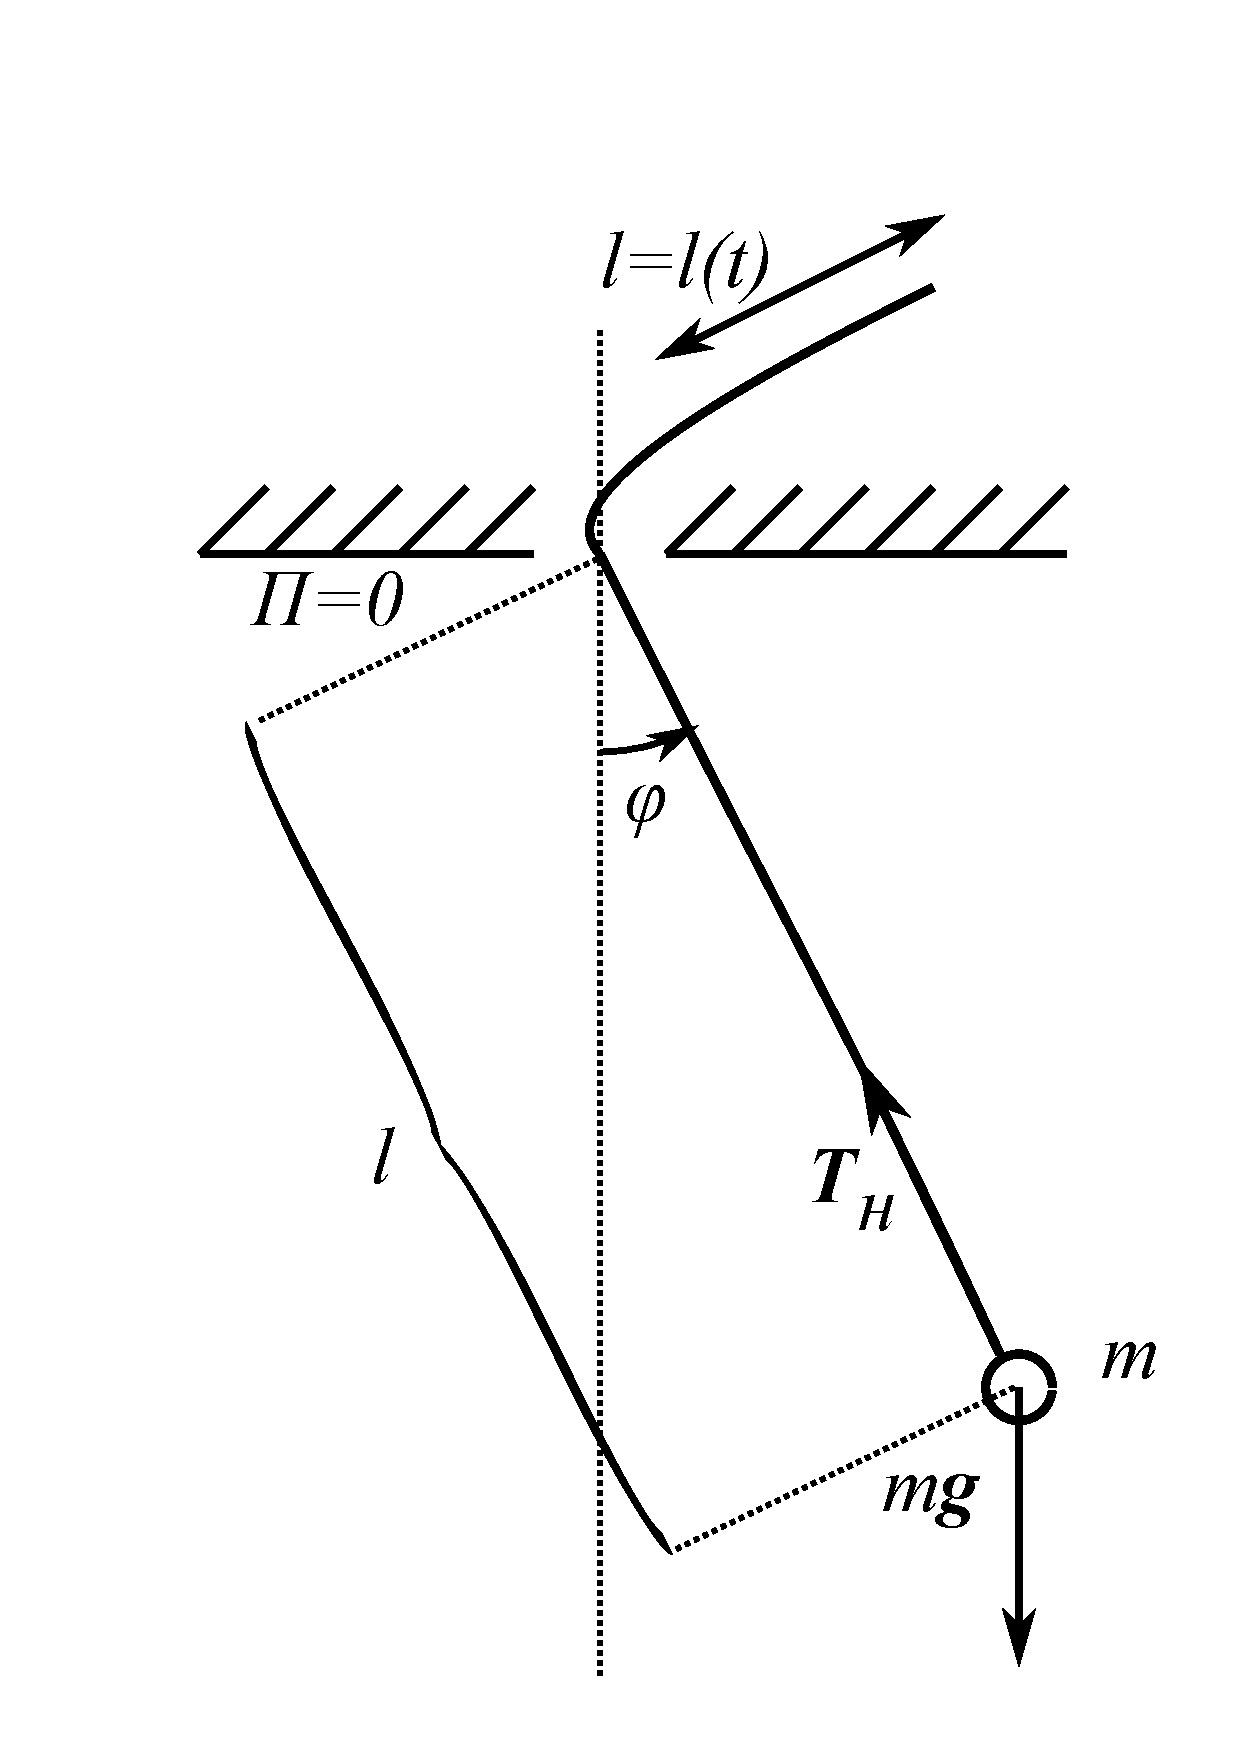
\includegraphics[width=\textwidth]{03}}
{
1) Груз обладает одной степенью свободы. Поэтому для описания его движения
достаточно одной координаты. Выберем в качестве координаты угол \( \phi \).

2) На груз действуют силы тяжести \( m\vec{g} \) и натяжения нити
\( \vec{T}_{\text{н}} \). Но сила натяжения нити работы не совершает
(перпендикулярна возможным перемещениям) -- связи идеальные. Поэтому можно
применить уравнение Лагранжа 2-го рода.

3) Потенциальная энергия, отсчитываемая от места закрепления нити
\[
    \Pi = - mgl(t) \cos \phi.
\]
    
4) Кинетическая энергия
\[
    T = \frac{mv^2}{2} = \frac{1}{2} m(l^2 \dot{\phi}^2 + \dot{l}^2).
\]
}

5) Уравнение Лагранжа:
\[
    ml^2\ddot{\phi} + 2 m l \dot{l} \dot{\phi} + m g l \sin \phi = 0
\]
или
\[
    \ddot{\phi} +  \frac{2\dot{l}}{ l}  \dot{\phi} +\frac{g}{ l} \sin \phi = 0.
\]

\newpage
